\documentclass{beamer}

\usepackage{emoji}
\usepackage{pgfplots}

\usetheme{UiO}

\title{SMBers rolle i å fylle implementeringsgapet innen AI og helse}
\author{Esten H. Leonardsen}
\date{06.03.2024}

\titlegraphic{
	\centering
	\vspace{7.7cm}
	
\includegraphics[width=\logowidth]{data/uio_logo_full.png}
}

\usetikzlibrary{arrows}
\usetikzlibrary{arrows.meta}
\usetikzlibrary{calc}
\usetikzlibrary{fadings}
\usetikzlibrary{fillbetween}
\usetikzlibrary{patterns}
\usetikzlibrary{positioning}
\usetikzlibrary{shapes.arrows}

\begin{document}
	\begin{frame}
	 	\titlepage
	\end{frame}

    \newcommand{\stickman}[2]{
        \node[circle,fill,minimum size=2.5mm,#2] (head) at #1 {};
        \node[rounded corners=1pt,minimum height=0.65cm,minimum width=0.2cm,fill,below = 0.5pt of head,#2] (body) {};
        \draw[line width=0.5mm,round cap-round cap,#2] ([shift={(1pt,-0.5pt)}]body.north east) --++(-90:3mm);
        \draw[line width=0.5mm,round cap-round cap,#2] ([shift={(-1pt,-0.5pt)}]body.north west)--++(-90:3mm);
        \draw[thick,white,-round cap] (body.south) --++(90:2.75mm);
    }


    \newcommand{\population}{
        \begin{tikzpicture}
            \node [
                double arrow,
                left color=blue,
                right color=red,
                double arrow head extend=0pt,
                transform shape,
                minimum height=1.5cm,
                text width=2.6cm,
                anchor=west
            ] at (-0.5, -1.25){};
            \node[font=\tiny, text=white] at (1.08, -1.25) {Symptomnivå};
            \stickman{(0, 0)}{blue}
            \stickman{(0.5, -0.1)}{blue}
            \stickman{(0.1, 1.1)}{blue}
            \stickman{(0.7, 1.05)}{blue}
            \stickman{(1.15, 0.1)}{blue}
            \stickman{(1.8, 0.2)}{blue!50!red}
            \stickman{(0.4, 2.2)}{blue!80!red}
            \stickman{(1.3, 1.4)}{blue!60!red}
            \stickman{(1.8, 2.2)}{blue!20!red}
            \stickman{(2.3, 1.2)}{blue!10!red}
        \end{tikzpicture}
    }

    \begin{frame}{Implementeringsgapet}
        \begin{tikzpicture}
            \node[draw=black] at (-5.25, -3.5) {};
            \node[draw=black] at (5.25, 3.5) {};

            \visible<1>{
                \node[label={[yshift=0.05cm]below:\tiny{Bilde generert av ChatGPT}}, inner sep=0pt] (brain) at (-3, 0) {
                    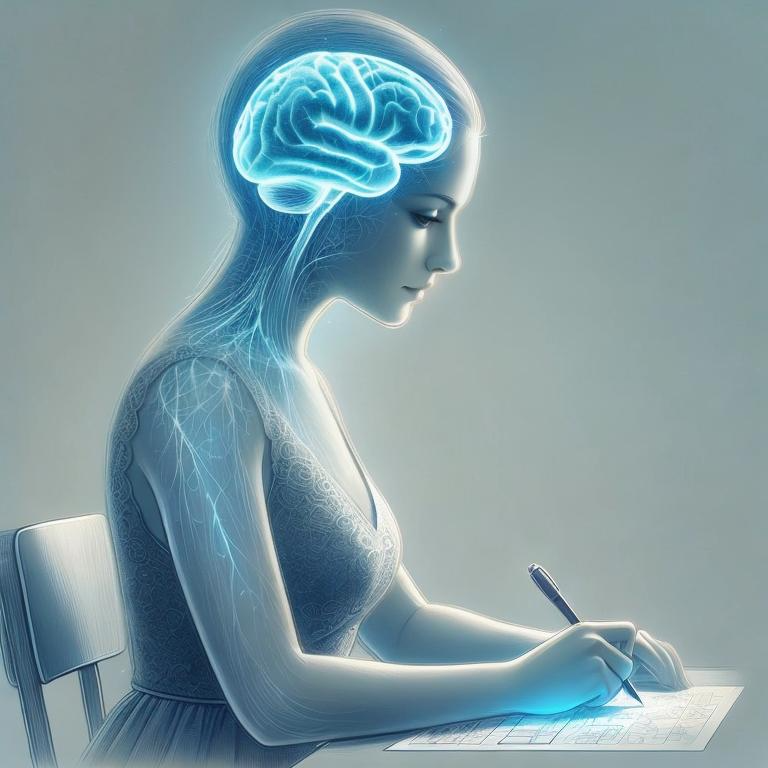
\includegraphics[width=3.5cm]{data/thinking.png}
                };
                \node[] (population) at (3, 0) {
                    \population
                };
                \draw[-stealth, line width=5pt, black!40] (brain) -- (population);
            }
            \visible<2-3>{
                \node[label={[yshift=-0.05cm]above:\footnotesize{27 år}}, inner sep=0pt] (input) at (-1.5, 2.5) {
                    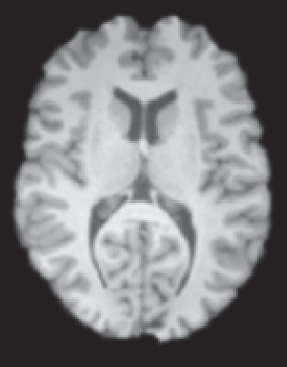
\includegraphics[height=1.5cm]{data/input.png}
                };
                \node[font=\fontsize{40}{25}] (notes) at (1.5, 2.5) {
                    \emoji{ledger}
                };
                \node[font=\tiny\linespread{0.9}\selectfont, align=center, text width=10cm, anchor=south] at (0, -3.75) {
                    Xia, T., Chartsias, A., Wang, C., Tsaftaris, S. A., \& Alzheimer’s Disease Neuroimaging Initiative. (2021). Learning to synthesise the ageing brain without longitudinal data. \textit{Medical Image Analysis}.
                };
            }
            \visible<3>{
                \node[align=center, font=\normalfont\linespread{0.9}\selectfont, draw=black, fill=teal!20, rounded corners=0.1cm, inner sep=5pt] (model) at (0, 0.5) {
                    Generativ\\kunstig intelligens
                };
                \node[label={[yshift=0.1cm]below:\footnotesize{37 år}}, inner sep=0pt] (output37) at (-2.5, -1.8) {
                    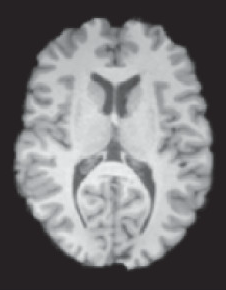
\includegraphics[height=1.5cm]{data/output_37.png}
                };
                \node[label={[yshift=0.1cm]below:\footnotesize{57 år}}, inner sep=0pt] (output57) at (0, -1.8) {
                    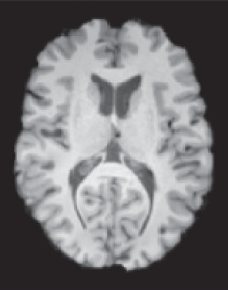
\includegraphics[height=1.5cm]{data/output_57.png}
                };
                \node[label={[yshift=0.1cm]below:\footnotesize{77 år}}, inner sep=0pt] (output77) at (2.5, -1.8) {
                    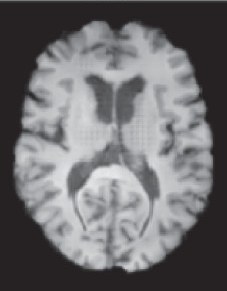
\includegraphics[height=1.5cm]{data/output_77.png}
                };

                \draw[-stealth, line width=2pt, gray] (input) to [out=270, in=90] ($ (model.north) - (0.125, 0) $);
                \draw[-stealth, line width=2pt, gray] ($ (notes.south) + (0, 0.08) $) to [out=270, in=90] ($ (model.north) + (0.125, 0) $);
                \draw[-stealth, line width=2pt, gray] (model) to [out=270, in=90] (output37);
                \draw[-stealth, line width=2pt, gray] (model) to [out=270, in=90] (output57);
                \draw[-stealth, line width=2pt, gray] (model) to [out=270, in=90] (output77);
            }
        \end{tikzpicture}
    \end{frame}

\end{document}
